\section{Data and Simulated Lead Failure}
\label{sec:data}

\subsection{PTB-XL}
\label{sec:data-ptbxl}
We use PTB-XL version~1.0.3 \citeneeded{PTB-XL dataset paper (Wagner et al.) and PhysioNet v1.0.3 record, DOI
10.13026/kfzx-aw45}, a public collection of clinical 12-lead ECGs of 10\,s each, annotated with SCP-ECG
statements. We use the 100\,Hz release, so every record is a $12\times1000$ array in the fixed lead order I, II,
III, aVR, aVL, aVF, V1--V6. Labels are the five diagnostic superclasses: normal ECG (NORM), myocardial infarction
(MI), ST/T change (STTC), conduction disturbance (CD) and hypertrophy (HYP). Every statement marked as diagnostic
is mapped to its superclass irrespective of its likelihood value, records may carry several superclasses
(multi-label), and records without any diagnostic superclass are excluded, leaving \nRecordsKept{} records. We follow the dataset's recommended stratified folds \citeneeded{PTB-XL paper
on \texttt{strat\_fold}}: folds 1--8 for training, fold~9 for validation and fold~10 (\nTestRecords{} records) for
testing. Each lead of each record is standardised to zero mean and unit variance; a lead whose standard deviation
is below $10^{-6}$ (a dead lead) is set to zero instead of being divided by a near-zero number. The raw
millivolt signal is kept only for display.

\subsection{A severity model of lead failure}
\label{sec:data-failure}
Every corruption acts on a batch $\mathbf{x}\in\mathbb{R}^{B\times12\times T}$ and returns the corrupted signal
together with a per-lead \emph{severity} $s_j\in[0,1]$, where $s_j=0$ means the lead is untouched (exactly) and
$s_j=1$ means it carries no usable signal. Severity defines the ground truth for the quality assessor,
$q^\ast_j=1-s_j$, and the binary label ``reliable'' $\Leftrightarrow s_j<0.5$. Five failure types are simulated
(Fig.~\ref{fig:corruptions}):
\begin{itemize}\setlength{\itemsep}{1pt}
  \item \emph{Removal}: the lead is set to zero ($s_j=1$), as when an electrode detaches.
  \item \emph{Flatline}: the lead holds its first sample, as with a stuck amplifier ($s_j=1$).
  \item \emph{Muscle (EMG) noise}: white noise band-limited to 20--45\,Hz in the Fourier domain and scaled to a
        target signal-to-noise ratio relative to the lead's own power; $s_j=1-\mathrm{clip}(\mathrm{SNR}_{\mathrm{dB}}/20,0,1)$.
        Mains interference (50/60\,Hz) is deliberately not simulated: it lies at or above the Nyquist frequency of
        the 100\,Hz signal and cannot be represented.
  \item \emph{Baseline wander}: a sinusoid of 0.1--0.5\,Hz with an amplitude of 0.5--3 times the lead's standard
        deviation, as from respiration or movement; $s_j=\mathrm{clip}(r/2,0,1)$ for amplitude ratio $r$.
  \item \emph{Amplitude clipping}: saturation at a percentile (70--95) of $|x|$; $s_j$ is the clipped fraction
        divided by 0.2, capped at~1.
\end{itemize}

\begin{figure*}[t]
\centering
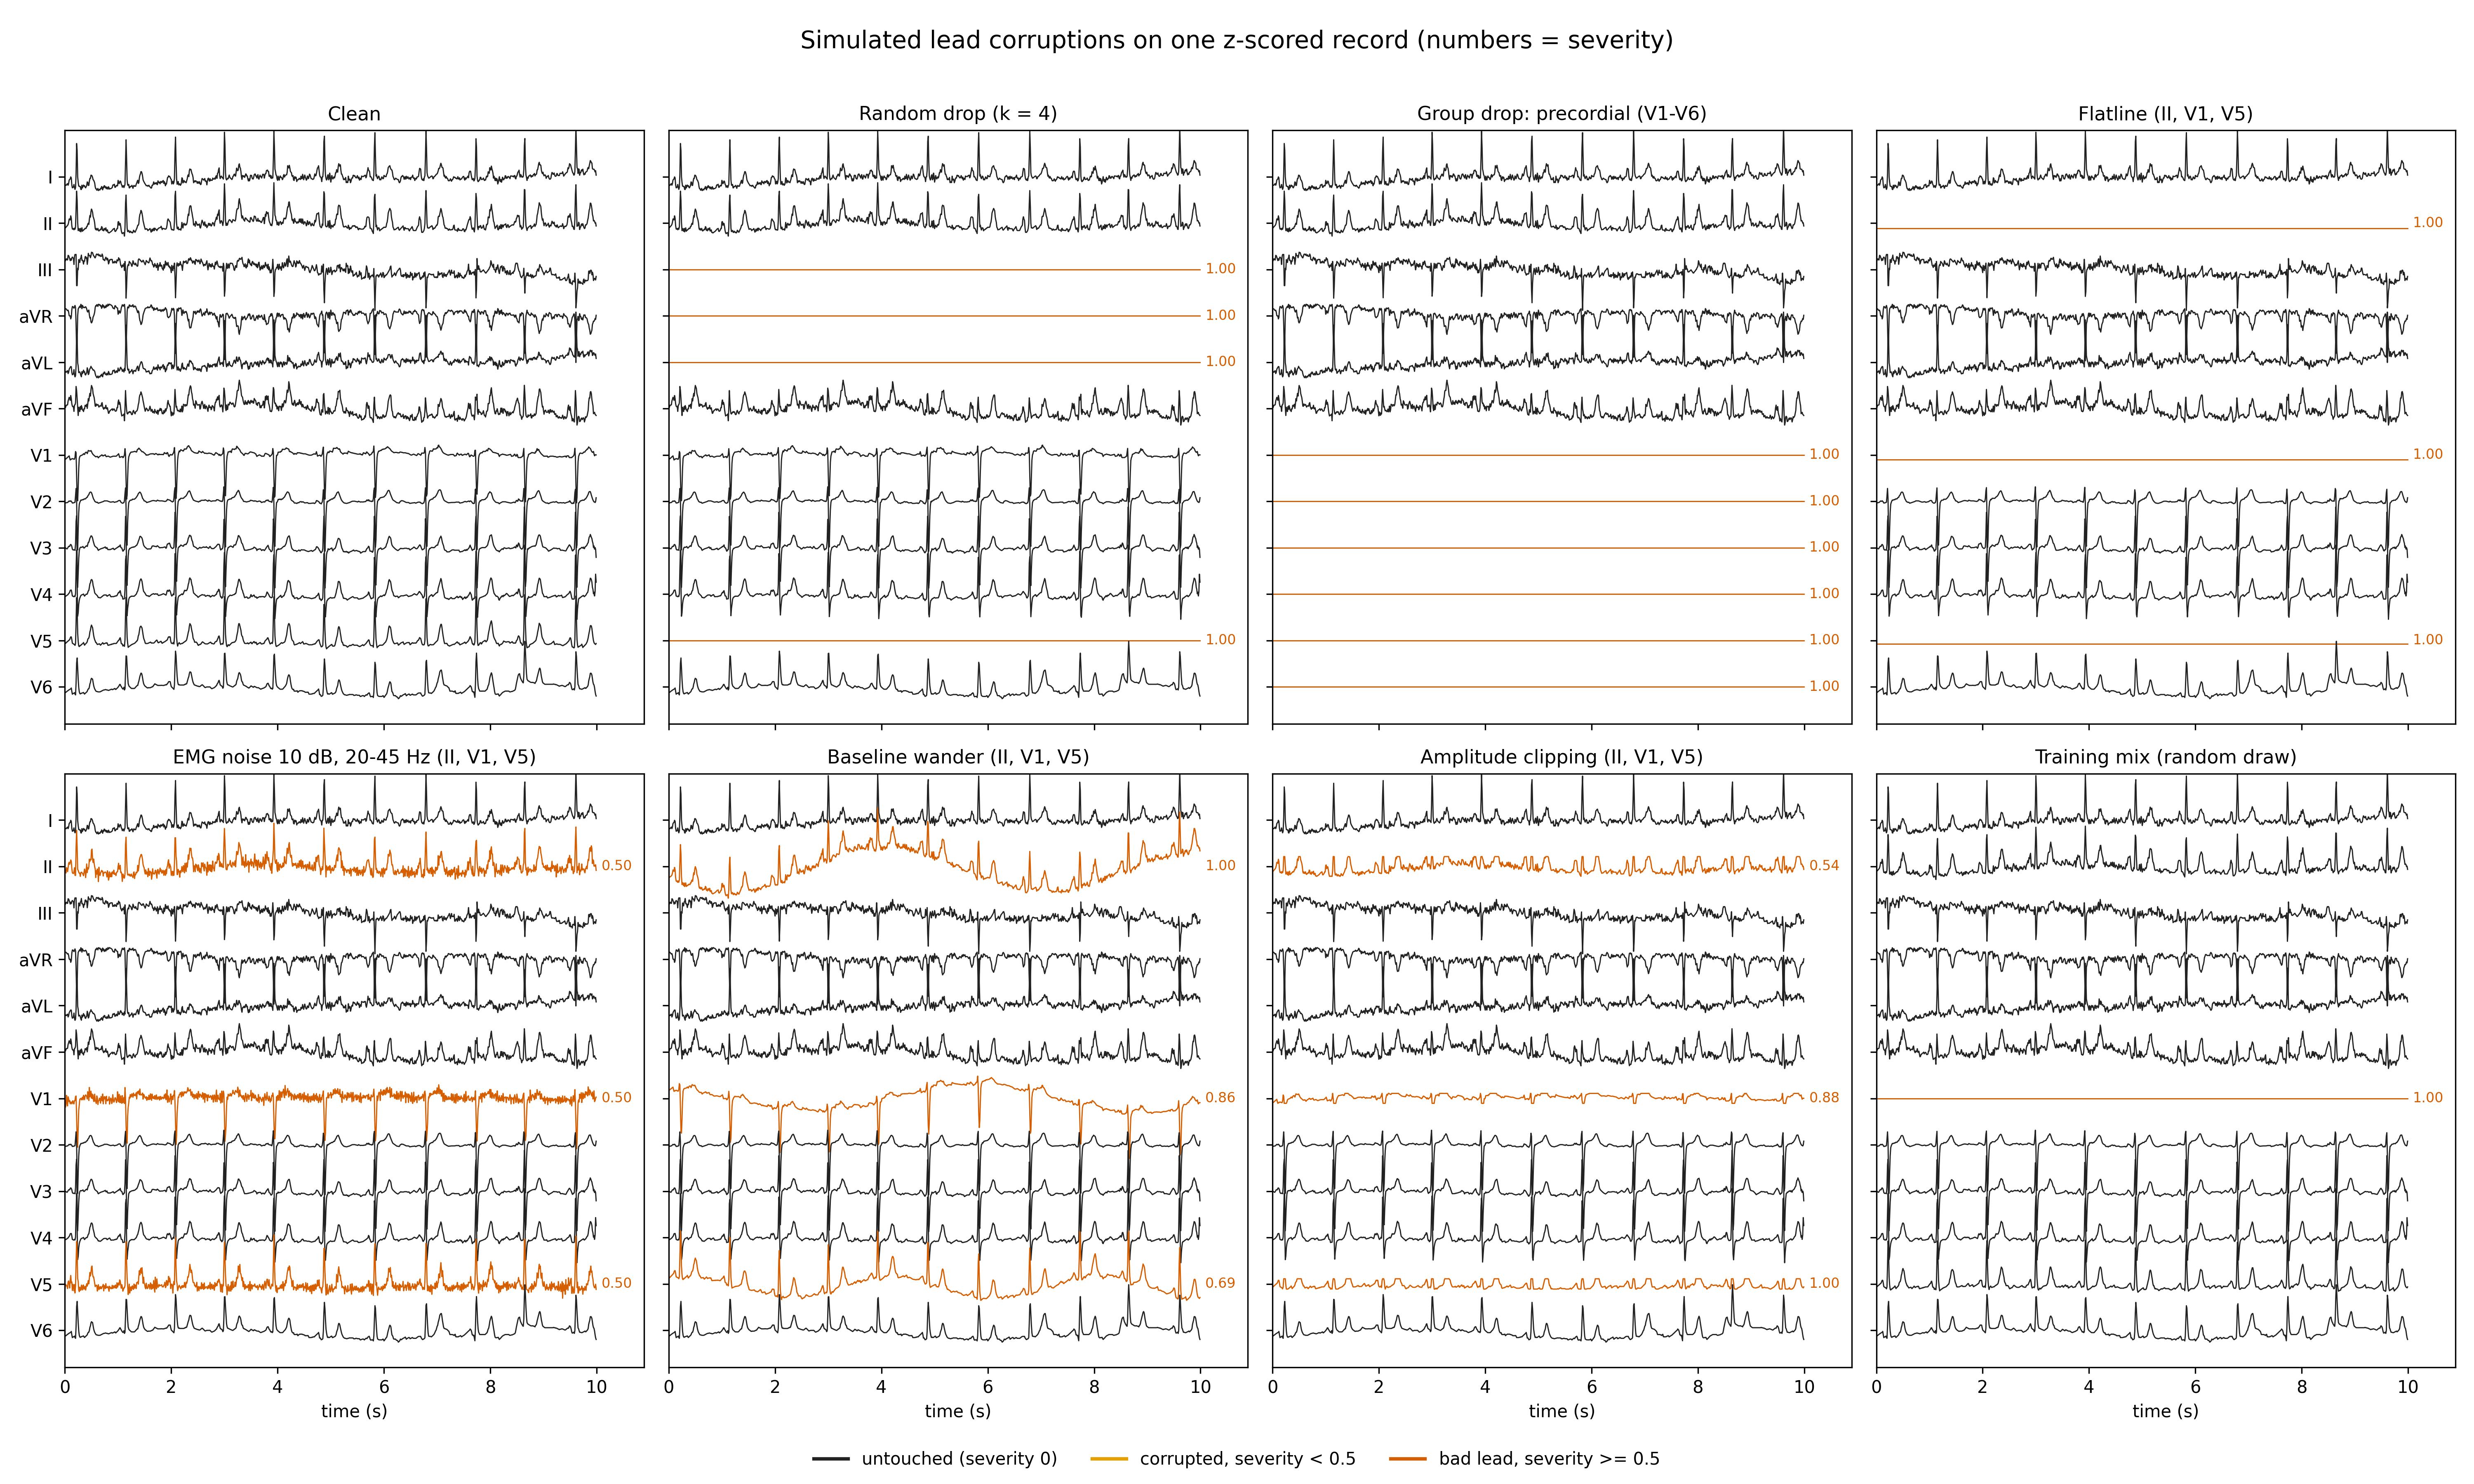
\includegraphics[width=0.92\textwidth]{corruption_examples.png}
\caption{The simulated failure types applied to one PTB-XL record (z-scored). Numbers give each lead's severity
$s_j$; black leads are untouched ($s_j=0$), light-orange leads are corrupted but still counted as reliable
($s_j<0.5$), dark-orange leads are unreliable ($s_j\ge0.5$). The last panel is one random draw of the training
mixture.}
\label{fig:corruptions}
\end{figure*}

\subsection{Training-time corruption}
\label{sec:data-train}
During training, corruption is sampled independently for every record of every batch. With probability 0.30 an
artifact (EMG noise with an SNR drawn uniformly from 0--20\,dB, baseline wander or clipping) is applied to one to
three random leads; with probability 0.50, zero to six random leads are removed, a quarter of them by flatlining
instead of zeroing; with probability 0.15, an entire lead group is removed (all precordial leads, all limb leads,
or V1--V3). These events can combine, artifacts are applied before removals, and the severity of a lead hit
twice is the larger of the two. If fewer than two reliable leads would remain, the least-corrupted leads are
restored, so every training record keeps at least two.

\subsection{Test-time conditions}
\label{sec:data-test}
For evaluation, the whole test fold is corrupted once per condition, on the CPU, with a random generator seeded
by the condition's name and draw, so that every model sees bit-identical inputs. The conditions are: the clean test
fold; random removal of $k\in\{0,2,4,6,8,10\}$ leads, three independent draws each; removal of the precordial
leads (V1--V6), the limb leads (I, II, III, aVR, aVL, aVF) or V1--V3; and EMG noise at 10\,dB, baseline wander or
clipping on two, four or six random leads. That makes 31 conditions including the clean one. EMG at 10\,dB has a
severity of exactly 0.5, on the boundary of the reliable label; we keep it because it is the realistic
operating point, and report the quality assessor's agreement both with and without such ambiguous leads
(Section~\ref{sec:setup}).
